\usecase{visualizzaRuoliPerTipoDocumento}{Visualizza ruoli disponibili per tipo di documento}
\begin{figure}[H]
      \centering
      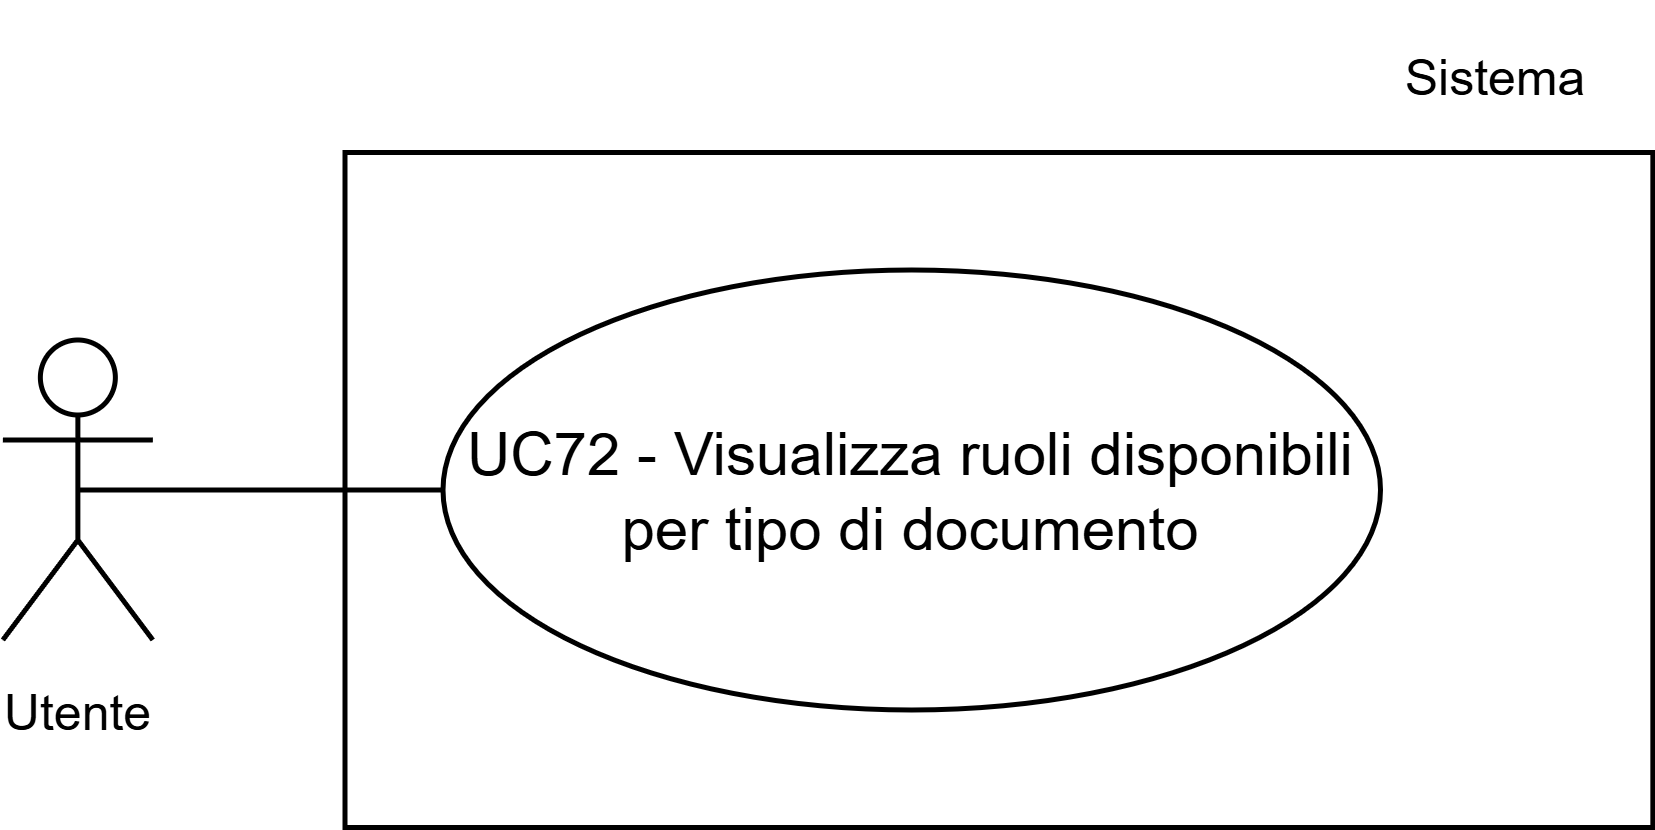
\includegraphics[width=0.5\textwidth]{../../assets/uml/UC72.png}
      \caption{\ref{visualizzaRuoliPerTipoDocumento} - Visualizza ruoli disponibili per tipo di documento}
      \label{fig:uc_visualizzaRuoliPerTipoDocumento}
\end{figure}
\begin{itemize}
      \item \textbf{Attore Primario}: Utente
      \item \textbf{Precondizioni}: 
      \begin{itemize}
            \item L'Utente ha avviato l'applicazione
            \item L'Utente ha specificato il filtro Tipo di Documento
      \end{itemize}
      \item \textbf{Postcondizioni}: Vengono mostrati i ruoli disponibili in base alla specifica del filtro Tipo di Documento.
      \item \textbf{Flusso Principale}:
            \begin{enumerate}
                  \item Il sistema mostra per ogni ruolo disponibile in base alla specifica del filtro Tipo di Documento:
                        \begin{itemize}
                              \item Nome del Ruolo (\ref{visualizzaNomeRuolo})
                        \end{itemize}
            \end{enumerate}
      \item \textbf{Inclusioni}: \ref{visualizzaNomeRuolo} Visualizza nome del ruolo
\end{itemize}
\begin{figure}[H]
      \centering
      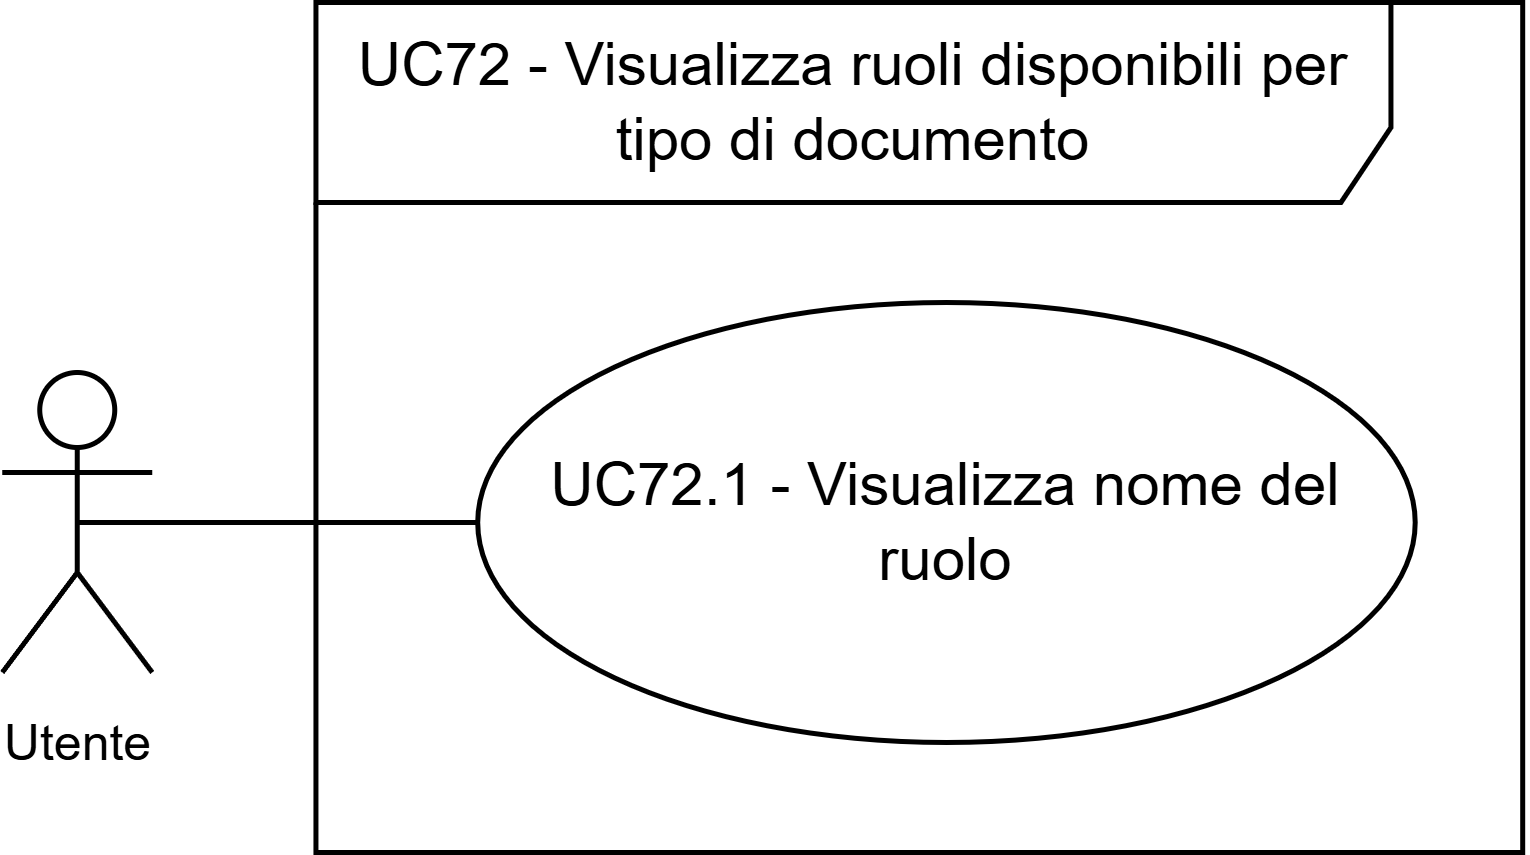
\includegraphics[width=0.5\textwidth]{../../assets/uml/UC72INC.png}
      \caption{Inclusioni \ref{visualizzaRuoliPerTipoDocumento} - Visualizza ruoli disponibili per tipo di documento}
      \label{fig:inclusioniVisualizzaRuoliPerTipoDocumento}
\end{figure}

\subusecase{visualizzaNomeRuolo}{Visualizza nome del ruolo}
\begin{itemize}
      \item \textbf{Attore Primario}: Utente
      \item \textbf{Precondizioni}:
      \item \begin{itemize}
            \item L'Utente ha avviato l'applicazione
            \item L'Utente sta visualizzando una lista di ruoli.
      \end{itemize}
      \item \textbf{Postcondizioni}: L'Utente visualizza il nome del ruolo.
      \item \textbf{Flusso Principale}:
      \item \begin{enumerate}
            \item Il sistema mostra a video il nome del ruolo.
      \end{enumerate}
\end{itemize}

\usecase{visualizzaTipiSoggettoPerRuolo}{Visualizza tipi di soggetto disponibili per ruolo}
\begin{figure}[H]
      \centering
      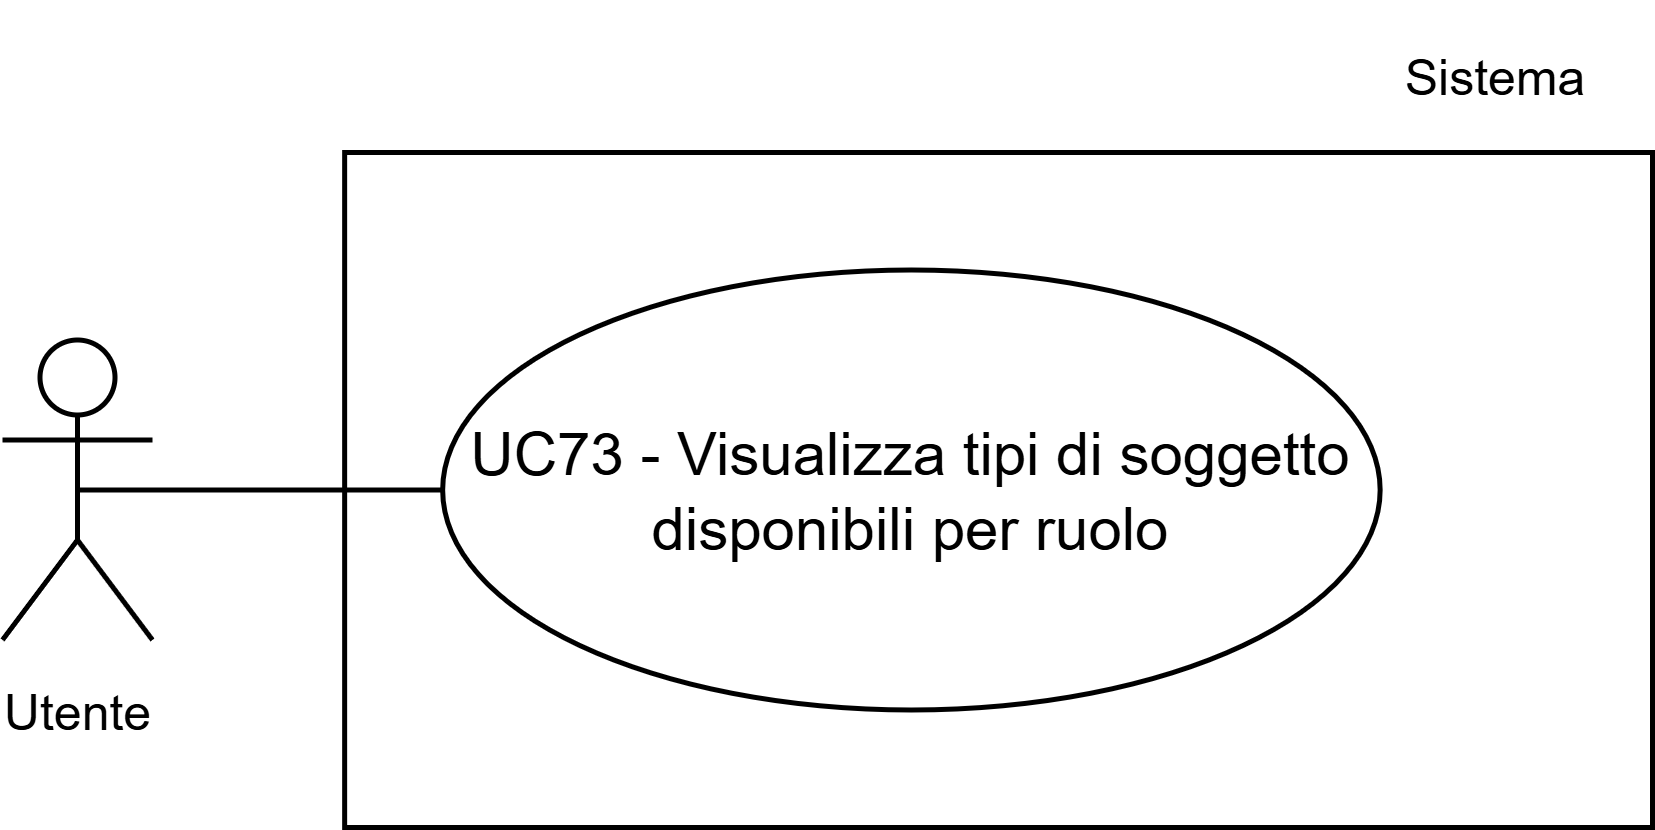
\includegraphics[width=0.5\textwidth]{../../assets/uml/UC73.png}
      \caption{\ref{visualizzaTipiSoggettoPerRuolo} - Visualizza tipi di soggetto disponibili per ruolo}
      \label{fig:uc_visualizzaTipiSoggettoPerRuolo}
\end{figure}
\begin{itemize}
      \item \textbf{Attore Primario}: Utente
      \item \textbf{Precondizioni}: 
      \begin{itemize}
            \item L'Utente ha avviato l'applicazione
            \item L'Utente sta aggiungendo un soggetto ad un filtro, di cui ne ha specificato il ruolo (\ref{specificaRuoloSoggetto})
      \end{itemize}
      \item \textbf{Postcondizioni}: Vengono mostrati i tipi di soggetto disponibili per il ruolo selezionato.
      \item \textbf{Flusso Principale}:
            \begin{enumerate}
                  \item Il sistema mostra, per ogni tipo di soggetto disponibile per il ruolo selezionato, il Nome del Tipo di Soggetto (\ref{visualizzaNomeTipoSoggetto})
            \end{enumerate}
      \item \textbf{Inclusioni}: \ref{visualizzaNomeTipoSoggetto} Visualizza nome del tipo di soggetto
\end{itemize}
\begin{figure}[H]
      \centering
      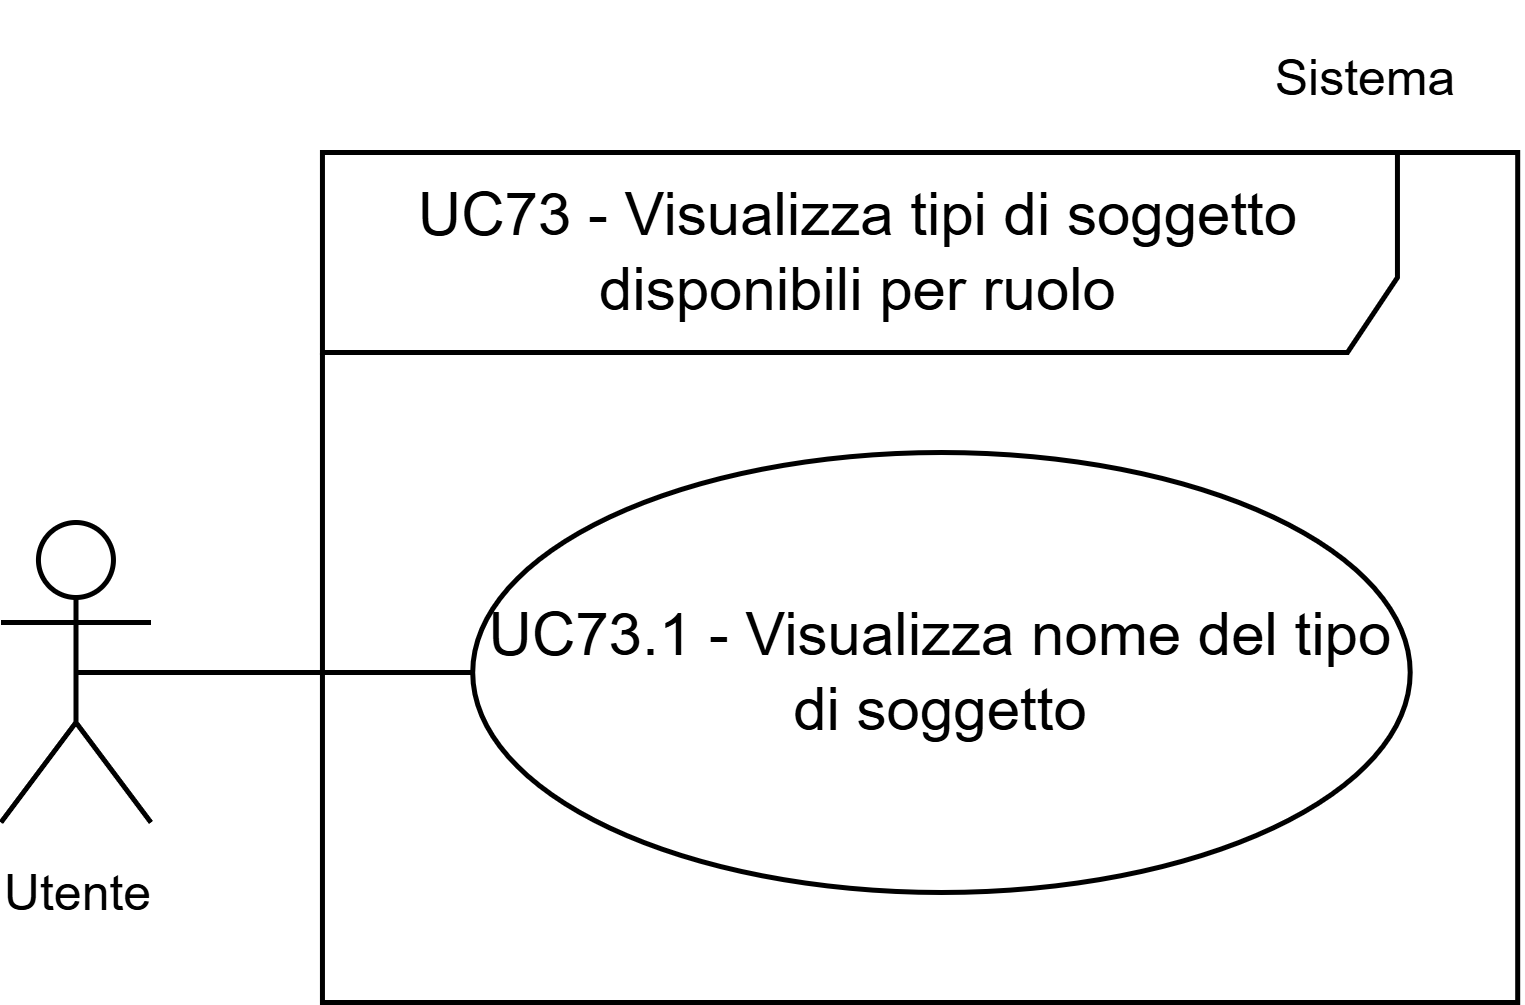
\includegraphics[width=0.5\textwidth]{../../assets/uml/UC73INC.png}
      \caption{Inclusioni \ref{visualizzaTipiSoggettoPerRuolo} - Visualizza tipi di soggetto disponibili per ruolo}
      \label{fig:inclusioniVisualizzaTipiSoggettoPerRuolo}
\end{figure}

\subusecase{visualizzaNomeTipoSoggetto}{Visualizza nome del tipo di soggetto}
\begin{itemize}
      \item \textbf{Attore Primario}: Utente
      \item \textbf{Precondizioni}:
      \item \begin{itemize}
            \item L'Utente ha avviato l'applicazione
            \item L'Utente sta visualizzando una lista di tipi di soggetto.
      \end{itemize}
      \item \textbf{Postcondizioni}: L'Utente visualizza il nome del tipo di soggetto.
      \item \textbf{Flusso Principale}:
      \item \begin{enumerate}
            \item Il sistema mostra a video il nome del tipo di soggetto.
      \end{enumerate}
\end{itemize}